\subsection{Factorisation forests}
\label{sec:factfor}
This section is devoted to stating and proving a tree version of the Factorisation Forest Theorem of Imre Simon.  Our result differs from the original Factorisation Forest Theorem in the following ways: (a) we consider trees instead of strings; (b) we use aperiodic finite monoids instead of arbitrary finite monoids; and (c) the factorisation in the conclusion of the theorem can be computed by a derivable function.  A tree generalisation of the Factorisation Forest Theorem was already proved by Colcombet~\cite[Theorem 1 and Section 3.3]{colcombetCombinatorialTheoremTrees2007}, but Colcombet's result is proved for monadic second-order logic, and therefore it does not satisfy condition (c). 



\paragraph{Factorisation forests} The idea behind factorisation forests is to split a term into a nested factorisation, which is a term of terms of terms, and so on up to a certain depth.  
Define a \emph{nested factorisation} of depth $k \in \set{1,2,\ldots}$ over alphabet $\rSigma$ to be an element of $\tmonadn k \rSigma$ which is defined by
\begin{align*}
\tmonadn 0 \rSigma = \rSigma  \quad \text{and} \quad \tmonadn {k+1}\rSigma = \tmonad \tmonadn k \rSigma.
\end{align*}
Nested factorisations can be flattened to terms by using an  operation $\flatn k : \tmonadn k \rSigma \rto \tmonad \rSigma $ defined by 
\begin{align*}
     \flatn 1 = \text{\ranked{identity}} \quad \text{and} \quad  \flatn {k+1} \eqdef \flatt  \circ \tmonad \redpar { \flatn k}.
\end{align*}
An equivalent definition of $\flatn {k+1}$ would be $\flatn k \circ \tmonadn {k-1} \flatt$, the equivalence of these definitions corresponds to the fact that $\tmonad$ is a monad.


\paragraph{Branches and subbranches}
Define a \emph{branch} in a ranked set to be an element  of the ranked set together with a distinguished port. 
We draw branches like  this:
\mypic{82}
We write $\branches \rSigma$ for the (unranked) set of branches over a ranked set $\rSigma$. \label{page:branches}
For a term, we classify its edges as internal (linking a non-port node with a non-port child) and external (linking a non-port node with a child port). Each edge in a term $t \in \tmonad \rSigma$ corresponds to a branch over $\rSigma$, namely the branch which leads to the edge. Any branch obtained this way is called a \emph{subbranch} of $t$. Here is a picture of subbranches in the case of a term of terms:
\mypic{80} 

\newcommand{\hb}[2]{#2^{(#1)}}
Branches in  terms  form a monoid. Using the monoid structure of branches in terms, we can extend any function  $h : \branches \rSigma \to M$, with $M$ a monoid, to a  monoid homomorphism
\begin{align*}
\hb n h : \branches \tmonadn n \rSigma \to M
\end{align*}
which maps a branch of a term to the product -- in the monoid $M$ -- of all of its subbranches (after flattening).  A more formal definition is that $\hb 0 h$ is the same as $h$, while  $\hb {n+1} h$  is the unique monoid homomorphism  which makes the following diagram commute
\begin{align*}
\xymatrix{
    \branches \tmonadn n \rSigma \ar[dr]^{\hb n h} \ar[d]_{\branches \unit}\\
    \ar[r]_{\hb {n+1}  h}\branches \tmonadn {n+1} \rSigma & M
}
\end{align*}


The idea behind factorisation forests, as expressed in Definition~\ref{def:hom-for} below, is to factorise a term into a term of terms of terms (etc.) so that the depth of nesting is bounded, and at each level all branches behave regularly with respect to some monoid homomorphism. 

\begin{definition}[Homogeneous factorisations]\label{def:hom-for}
    Let $h : \branches \rSigma \to M$ be a function into a monoid $M$. 
    \begin{itemize}
\item     We say that a factorisation $t \in \tmonad \tmonad \rSigma$ is \emph{homogeneous with respect to $h$} if it either:
\begin{enumerate}
    \item \label{it:factfor-shallow} it is a shallow term (which means that all internal edges originate from the root); or 
    \item \label{it:factfor-allsame} all internal subbranches of $t$ have the same value under $\hb 1 h$; or
    \item \label{it:factfor-ab} if $a,b \in M$ appear as values -- under $\hb 1 h$ -- of internal branches in $t$, then $ab=a$. 
\end{enumerate}
\item We say that a nested factorisation  $t \in \tmonadn n \rSigma$ is \emph{hereditarily homogeneous with respect to $h$} if either $n=1$ and $t$ is the unit of a letter, or $n \ge 2$ and both:
\begin{enumerate}
    \item  it is homogeneous with respect to $\hb {n-1} h$; and 
    \item every node has a label in $\tmonadn {n-1} \rSigma$ that is hereditarily homogeneous with respect to $h$.
\end{enumerate}
    \end{itemize}
\end{definition}


Recall that a finite monoid is aperiodic if it has only trivial subgroups. An equivalent definition is that every element $m$ of the monoid satisfies 
\begin{align*}
  \exists n \in \set{1,2,\ldots}\   m^n = m^{n+1}.
\end{align*} 
A famous theorem of Sch\"utzenberger, McNaughton and Papert, see~\cite[Theorem VI.1.1]{straubingFiniteAutomataFormal1994} says that the languages  of words recognised by homomorphisms into finite aperiodic monoids are exactly  those that can be defined in first-order logic. This is the reason why  we consider aperiodic monoids.

\begin{example}\label{ex:partial-monoton-functions}
   Let $k \in \set{1,\ldots}$ and  consider the monoid of partial functions 
    \begin{align*}
    \set{1,\ldots,k} \to \set{1,\ldots,k}.
    \end{align*}
    This monoid is not aperiodic, because it contains the  group of all permutations of $\set{1,\ldots,k}$. Consider now the restriction of this monoid to partial functions which are monotone (this is a monoid, because such functions are closed under composition). This monoid is aperiodic, because if $f$ is a partial function, then for  every $i \in \set{1,2,\ldots,k}$ the sequence
    \begin{align*}
    f^1(k),f^2(k),f^3(k),\ldots
    \end{align*}
    reaches a fixpoint (or becomes undefined) in at most $k$ steps.
\end{example}
We are now ready to state our version of the Factorisation Forest Theorem. 
\begin{theorem}[Factorisation Forest Theorem]\label{thm:factfor}
    Let $\rSigma$ be a  ranked set and let $h : \branches  \rSigma \to M$ be a function into a finite aperiodic monoid $M$. There is some $n \in \set{1,2,\ldots}$ and a  function
    \begin{align*}
        \ranked {f : \tmonad \rSigma \to \tmonad^n \rSigma}  
    \end{align*}
such that $\flatn n \circ \ranked f$ is the identity on $\tmonad \rSigma$, and  all outputs of  $\ranked f$ are hereditarily homogeneous with respect to $h$. Furthermore, if $\rSigma$ is finite\footnote{This finiteness assumption could be relaxed by saying that $\rSigma$ is possibly infinite but the function $h$ is derivable, in the sense that a derivable function can decorate the ports of an element in $\rSigma$ by their values under $M$.} then $\ranked f$ is derivable. 
\end{theorem}



\newcommand{\hint}{\bar h}
\newcommand{\hintplus}{\bar h^+}
\newcommand{\branchesplus}{\mathsf B^+}


% Later in this section, we also give a sufficient condition which ensures that $\ranked f$ as in the theorem is derivable, by analysing in more detail the proof the theorem. 
In the proof below, the constructions  are designed so that they can be formalised using derivable functions, however we leave the details of  the ``Furthermore'' part to the reader. 

Define a \emph{good set} to be any subset  $\ranked X \subseteq  \tmonad \rSigma$ which admits a function 
\begin{align*}
    \ranked {f : \tmonad \rSigma \to \tmonad^n \rSigma}   \qquad \text{for some $n \in \set{1,2,\ldots}$}
\end{align*}
such that $\flatn n \circ \ranked f$ is the identity on $\tmonad \rSigma$, and    $\ranked f$ restricted to $\ranked X$ produces only hereditarily homogeneous outputs. Our goal is to show that the entire set $\tmonad \rSigma$ is good. To prove this, we use a more refined result, stated below, which has a parameter  that can be used for  induction.  We say that a term $t \in \tmonad \rSigma$ uses $A \subseteq M$ for  internal subbranches if all  internal subbranch have image under $\hb 1 h$ that belongs to $A$. 

\begin{lemma}\label{lem:fact-ind}
    Let $\rSigma$ be a  ranked set and let $h : \branches \tmonad \rSigma \to M$ be a monoid homomorphism into a finite aperiodic monoid $M$. For every $A \subseteq M$, the  terms that use $A$ for inner subbranches  is good.
    \end{lemma}

\newcommand{\subgen}[1]{\langle #1 \rangle}
Theorem~\ref{thm:factfor} follows immediately from the  lemma, by taking $A$ to be the entire monoid. The rest of Section~\ref{sec:factfor} is therefore devoted to proving the lemma. The proof is by induction on  two parameters: (a) the size of $A$; and (b) 
the size of the semigroup $\subgen A \subseteq M$ that is  generated by $A$.
 These parameters are  ordered lexicographically, with the size of the semigroup being more important.

The induction base is when $A$ contains only one element $a$ of the monoid. If a term uses $\set a$ for  internal subbranches, then applying $\tmonad \unit$ leads to a factorisation that is  homogeneous according to item~\ref{it:factfor-allsame} of Definition~\ref{def:hom-for}, which is also hereditarily homogeneous because all nodes are labelled by units. This completes the proof of the induction base.

In the proof of the induction step, we consider two cases.
\begin{itemize}
    \item The first case is  when  every $a \in A$ satisfies 
    \begin{align*}
       \subgen{\set{ b a :  b \in \subgen A}} = \subgen A
  \end{align*}
  This means that every for every $a \in A$, the function $b \mapsto ba$ is a permutation of $\subgen A$. Since the monoid is aperiodic, this permutation must necessarily be the identity.  Therefore, we have $ab=a$ for every $a,b \in \subgen A$. This means that if all a term uses $A$ for  internal subbranches, then applying $\tmonad \unit$  gives a factorisation which is hereditarily homogeneous according to item~\ref{it:factfor-ab} of Definition~\ref{def:hom-for}. 
    \item If the previous item does not hold, then there is some $a \in A$ such that 
    \begin{align*}
         \subgen{\set{ b a :  b \in \subgen A}}
    \end{align*}
    is a proper subsemigroup of $\subgen A$.  Fix some such $a$.  Define a \emph{sensitive edge} in a term  $t \in \tmonad \rSigma$ to be any internal edge where the corresponding subbranch has value $a$ under  $\hb 1 h$. Call an internal edge \emph{post-sensitive} if it is not sensitive, but its parent edge is. Here is a picture:
    \begin{center}
\includegraphics[scale=.27, page=8]{pics}
\end{center}
    Define the \emph{split} of a term to be the factorisation which  cuts along post-sensitive  edges, as shown in the following picture:
    \begin{center}
\includegraphics[scale=.29, page=88]{pics}
\end{center}
    We only consider splits for terms which use $A$ for internal subbranches. Roughly speaking,  we will show that all factors in the split are good, and the split itself is good.  Combining these two observations, we will see that all terms 

    We begin by looking at the factors in the split (of a term where $A$ is used for internal subbranches). Here is a picture of such a factor:
    \mypic{89}
        If we follow a  branch in an factor of the split, from root to port, we first  have a sequence of non-sensitive  edges from the original term, followed by a sequence of sensitive edges. Group the non-sensitive edges together, and group the sensitive edges together, resulting in a shallow term from $\shallowterm{\tmonad \rSigma}{\tmonad \rSigma}$, which is illustrated in the following picture:
     \begin{center}
\includegraphics[scale=.3, page=90]{pics}
\end{center}
        In the resulting shallow term,  the root is labelled by a term without sensitive edges (i.e.~it is a term which uses $A - \set a$ for internal subbranches), while the children are labelled by terms where all edges are sensitive (i.e.~they are terms which use $\set a$ for internal subbranches). We can apply the induction in both cases, and combine the resulting nested factorisations using a shallow term, as in item~\ref{it:factfor-shallow} of Definition~\ref{def:hom-for}.

        Having established that the factors of the split are good, we turn to the split itself. By construction, every subbranch of the split is mapped by $\hb 1 h$ to the smaller semigroup 
        \begin{align*}
            \subgen{\set{ b a :  b \in \subgen A}},
       \end{align*}
       We can  view the  split as a term over alphabet $\rGamma = \tmonad \rSigma$.  Since all  internal subbranches of the split are in the smaller subsemigroup, we can apply the induction assumption of the lemma (with $\rGamma$ and $\hb 1 h$), showing that the split is good. More formally, the set 
       \begin{align*}
       \set{\text{split of $t$} : t \in \tmonad  \rGamma \text{ uses $A$ for internal subbranches}}
       \end{align*}
       is good. To show now that original set of terms $t$ that use $A$ for  internal branches is good, we first apply the split, then compute the nested factorisation for the split, and finally we compute the nested factorisations for the factors of the split (the letters from $\rGamma$.). 
\end{itemize}


% We now give a proof sketch of the ``Furthermore'' part in the theorem, which says that if $\rSigma$ is finite, then
% \begin{align*}
%     \ranked {f : \tmonad \rSigma \to \tmonad^k \rSigma}  
% \end{align*}
% in the conclusion of the theorem not only exists, but it is derivable. In the proof sketch, we will appeal to the power of first-order tree relabellings from Section~\ref{sec:fo-translation}. To use tree relabellings, define \emph{pseudo-flattening} to be the  function 
% \begin{align*}
% \ranked{\mathrm{pseudoflat}} : \tmonad \tmonad \rSigma \rto \tmonad\redpar{\rSigma \redplus \redset{\overbrace{\text{open},\text{close}}^{\text{arity 2}}}}
% \end{align*}
% which adds an ``open'' whenever a new factor starts and adds a ``close'' letter whenever a factor ends, as depicted in the following picture:
% \mypic{91}
% Pseudo-flattening can be lifted in a natural way to nested factorisations 
% \begin{align*}
%     \ranked{\mathrm{pseudoflat}_n : \tmonadn {n+1} \rSigma \rto \tmonad \Sigma_n} \qquad \text{where }\ranked{\Sigma_n} \eqdef \redpar{\rSigma \redplus \redset{\overbrace{{\text{open}_i,\text{close}_i }}^{\text{arity 2}: i \in \set{1,\ldots,n}}}}
% \end{align*}
% Call a function $\ranked f$  \emph{pseudo-derivable} if there  is a derivable $\ranked g$ which makes the following diagram commute
%     \begin{align*}
%     \ranked{
%         \xymatrix{
%             \tmonad \rSigma \ar[r]^f \ar[d]_{\mathrm{pseudoflat}}& \tmonadn n \rSigma \ar[d]^{\mathrm{pseudoflat_n}} \\
%             \tmonad \rSigma_1 \ar[r]_g & \tmonad \rSigma_n 
%         }
%     }
%     \end{align*}
    
% \begin{lemma}\label{lem:pseudo-der}
%     A function $\ranked f$ is derivable if and only if it is pseudo-derivable.    
% \end{lemma}
% \begin{proof}
%     (Sketch.) Pseudo-flattening and its nested extensions are  easily seen to be derivable, and the same is true for their (one-sided) inverses.  
% \end{proof}
 
% The advantage of  pseudo-flattening  is that it allows use to work with first-order tree relabellings, which are much easier to work with. By an analysing the proof of Lemma~\ref{lem:fact-ind}, one can show that if $\rSigma$ is finite, then  the function $\ranked f$ is pseudo-derivable. This is because the basic operations in the proof of the lemma, such as ``find the first sensitive edge'' can easily be formalised in first-order logic, which in turn can be turned into derivable functions by virtue of Proposition~\ref{prop:forat}. 